\documentclass[11pt]{article}
\usepackage{amsmath}
\usepackage{gensymb}
\usepackage{graphicx}
\usepackage{listings}
\usepackage{xcolor}
\usepackage{bodegraph}
\usepackage[margin=1in]{geometry}

% Set up for code listing
\lstset{
    language=Matlab,
    basicstyle=\ttfamily\small,
    keywordstyle=\color{blue},
    commentstyle=\color{green},
    morecomment=[l][\color{magenta}]{\#},
    frame=single,
    breaklines=true
}

\begin{document}
\title{ELCT 331 Control Systems Assignment 6}
\author{Jacob C. Vaught}
\date{December 14th, 2023}
\maketitle
\section*{Problem \#1 [20 points]}
For the following bode plot, read the crossover frequencies and gain/phase 
margins. Determine if the system is stable.

% Importing the root locus plot image
\begin{center}
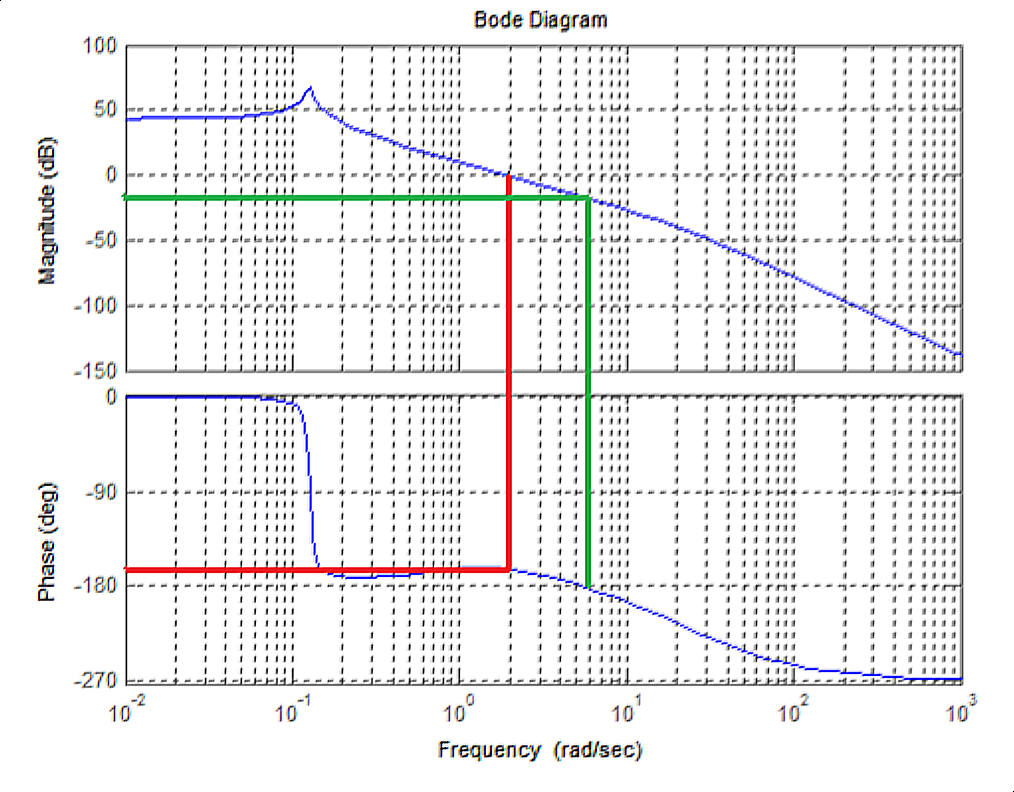
\includegraphics[width=0.8\textwidth]{HW6_1.png}
\end{center}


\newpage
\section*{Solution}
The phase crossover frequency, which is the frequency at which the phase plot crosses the \(-180^\circ\) line, is approximately \(6 \, \text{rad/sec}\). At this frequency, the magnitude is about \(-20 \, \text{dB}\).
\newline

The gain crossover frequency, which is the frequency at which the magnitude plot crosses the \(0 \, \text{dB}\) line, is approximately \(2 \, \text{rad/sec}\). At this frequency, the phase is about \(-160^\circ\).
\newline

The phase margin is calculated by adding \(180^\circ\) to the phase at the gain crossover frequency, which gives us:
\[
\text{Phase margin} = 180^\circ + (-160^\circ) = 20^\circ.
\]

The gain margin is found by subtracting the magnitude at the phase crossover frequency from \(0 \, \text{dB}\), resulting in:
\[
\text{Gain margin} = 0 \, \text{dB} - (-20 \, \text{dB}) = 20 \, \text{dB}.
\]

Since both the gain margin and the phase margin are positive, the system is considered to be stable.

\newpage
\section*{Problem \#2 [20 points]}
Find the magnitude-frequency and phase-frequency characteristics of \( G(s) = \frac{10}{s-2} \). Calculate the magnitude and phase at \( \omega = 1, 20, 500 \) rad/sec.

\section*{Solution}
Given the transfer function:
\[
G(j\omega) = \frac{10}{j\omega - 2} = \frac{-20 - j10\omega}{\omega^2 + 4}
\]
To find the magnitude \( |G(j\omega)| \) and phase \( \angle G(j\omega) \), we use the following equations:
\newline
\newline
The magnitude is given by:
\[
|G(j\omega)| = \frac{10}{\sqrt{\omega^2 + 4}}
\]
And the phase \( \angle G(j\omega) \) is calculated by:
\[
\angle G(j\omega) = \arctan\left(\frac{-10\omega}{-20}\right) = \arctan\left(0.5\omega\right)
\]
Since the real part of the denominator is negative and the imaginary part is also negative, the complex number \( -20 - j10\omega \) lies in the third quadrant. Therefore, the angle from the arctangent must be adjusted by adding \( 180^\circ \) to get the correct phase angle for the third quadrant.
\newline\newline
So, the phase is given by:
\[
\angle G(j\omega) = 180^\circ + \arctan\left(0.5\omega\right)
\]
Now we calculate the magnitude and phase for specific values of \( \omega \):

1. At \( \omega = 1 \) rad/sec:
\[
|G(j\omega)|_{\omega=1} = 4.472; \quad \angle G(j\omega)_{\omega=1} = 180^\circ + \arctan\left(0.5 \cdot 1\right) = 153.4^\circ
\]

2. At \( \omega = 20 \) rad/sec:
\[
|G(j\omega)|_{\omega=20} = 0.4975; \quad \angle G(j\omega)_{\omega=20} = 180^\circ + \arctan\left(0.5 \cdot 20\right) = 95.7^\circ
\]

3. At \( \omega = 500 \) rad/sec:
\[
|G(j\omega)|_{\omega=500} = 0.02; \quad \angle G(j\omega)_{\omega=500} = 180^\circ + \arctan\left(0.5 \cdot 500\right) = 90.2^\circ
\]


\newpage
\section*{Problem \#3 [30 points]}
The forward path of a unity feedback system is given by
\[
G(s) = \frac{K}{s(Ts+1)},
\]
with input \( r(t) = \sin(10t) \), the steady state output of the feedback system is \( y(t) = \sin(10t - 90^\circ) \). Please determine the values of \( K \) and \( T \).

\section*{Solution}
% Define the system transfer function
The closed-loop transfer function for the system is given by:
\[
M(s) = \frac{K}{Ts^2 + s + K}
\]
% Define the frequency response
The frequency response \( M(j\omega) \) at a specific frequency \( \omega \) is found by replacing \( s \) with \( j\omega \):
\[
M(j\omega) = \frac{K}{T(j\omega)^2 + j\omega + K}
\]
% Simplify the frequency response
Simplify the expression by separating the real and imaginary parts:
\[
M(j\omega) = \frac{K}{-T\omega^2 + j\omega + K}
\]
% Define the magnitude and phase of the frequency response
The magnitude \( |M(j\omega)| \) is given by:
\[
|M(j\omega)| = \frac{K}{\sqrt{(K - 10T)^2 + 100}}
\]
and the phase \( \angle M(j\omega) \) is given by:
\[
\angle M(j\omega) = -\arctan\left(\frac{10}{K - 10T}\right)
\]
% Establish the conditions based on the steady-state output
At \( \omega = 10 \) rad/sec, we want the system to have a magnitude of 1 and a phase lag of \( -90^\circ \). This gives us two conditions:
\[
\sqrt{(K - 100T)^2 + 100} = K
\]
\[
-\arctan\left(\frac{10}{K - 100T}\right) = -90^\circ
\]
% Solve for T and K using the phase condition
The phase condition implies that \( K - 100T = 0 \), which means \( K = 100T \). The arctan of an infinite value is \( 90^\circ \), and for a phase lag of \( -90^\circ \), the denominator must approach 0, thus:
\[
-\arctan\left(\frac{10}{0^+}\right) = -90^\circ
\]
% Solve for T and K using the magnitude condition
Substituting \( K = 100T \) into the magnitude condition, we get:
\[
\sqrt{(100T - 100T)^2 + 100} = 100T
\]
\[
\sqrt{100} = 100T
\]
\[
10 = 100T
\]
\[
T = 0.1
\]
% Determine the value of K
Finally, substituting \( T = 0.1 \) back into \( K = 100T \), we find:
\[
K = 100 \times 0.1 = 10
\]
% Provide the final values
Therefore, the values of \( K \) and \( T \) that satisfy the steady-state output are:
\[
K = 10, \quad T = 0.1
\]
\newpage
\section*{Problem \#4 [30 points]}
Roughly sketch the Nyquist plot of the transfer function 
\[
G(s) = \frac{2}{s(s^2 + 30s + 20)},
\]
calculate the gain and phase margins, and determine if the system is stable.

\section*{Solution}

Given the transfer function in the Laplace domain:
\[ G(s) = \frac{2}{s(s^2 + 30s + 20)} \]
Substituting \( s = j\omega \) to find the frequency response \( G(j\omega) \):
\[ G(j\omega) = \frac{250}{(j\omega)^3 + 30(j\omega)^2 + 20j\omega} \]
\[ G(j\omega) = \frac{250}{-30\omega^2 - j(\omega^3 - 20\omega)} \]
Multiplying both numerator and denominator by the conjugate of the denominator:
\[ G(j\omega) = \frac{250(-30\omega^2 + j(\omega^3 - 20\omega))}{(-30\omega^2 - j(\omega^3 - 20\omega))(-30\omega^2 + j(\omega^3 - 20\omega))} \]
\[ G(j\omega) = \frac{-7500\omega^2 + j(250\omega^3 - 5000\omega)}{\omega^6 + 860\omega^4 + 400\omega^2} \]
For the gain crossover frequency (\( \omega_g \)):
\[ \left|\frac{250}{\sqrt{(-30\omega^2)^2 + (\omega^3 - 20\omega)^2}}\right| = 1 \]
Solving the equation for \( \omega_g \):
\[ \omega^6 + 860\omega^4 + 400\omega^2 - 250^2 = 0 \]
\[ \omega_g \approx 2.87 \text{ rad/sec} \]
For the phase crossover frequency (\( \omega_p \)), the imaginary part should be zero:
\[ 250\omega^3 - 5000\omega = 0 \]
\[ \omega_p = 0 \text{ or } \omega_p = 4.47 \text{ rad/sec} \]
Calculating the magnitude at \( \omega = 4.47 \) rad/sec:
\[ |G(j\omega)|_{\omega=4.47} = \frac{250}{\sqrt{(-30\cdot 4.47)^2 + (4.47^3 - 20\cdot 4.47)^2}} \]
\[ |G(j\omega)|_{\omega=4.47} \approx 0.4171 \]
The gain margin (GM) is calculated as:
\[ \text{GM} = 0 - 20\log_{10}(0.4171) \approx 7.6 \text{ dB} \]
Calculating the phase at \( \omega = 2.87 \) rad/sec:
\[ \angle G(j\omega)|_{\omega=2.87} = 0 - 90^\circ - \arctan\left(\frac{30\cdot 2.87}{20 - 2.87^2}\right) \]
\[ \angle G(j\omega)|_{\omega=2.87} \approx -172.2^\circ \]
The phase margin (PM) is then:
\[ \text{PM} = 180^\circ + (-172.2^\circ) \approx 7.8^\circ \]
Since GM \> 0 and PM \> 0, the system is stable.
\newline\newline
To sketch the Nyquist plot, consider the following points:
At \( \omega = 0 \):
\[ |G(j\omega)|_{\omega=0} = \infty \]
\[ \angle G(j\omega)|_{\omega=0} = -90^\circ \]
At \( \omega = \infty \):
\[ |G(j\omega)|_{\omega=\infty} = 0 \]
\[ \angle G(j\omega)|_{\omega=\infty} = -270^\circ \]

% Importing the root locus plot image
\begin{center}
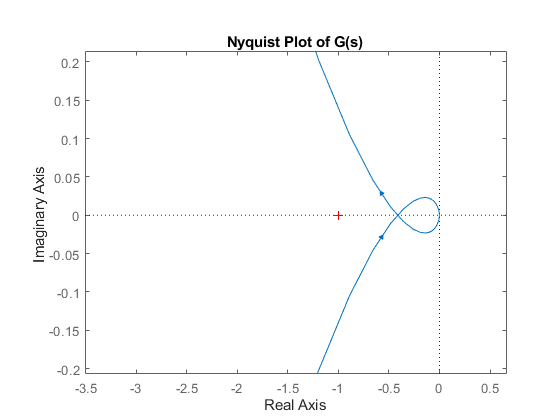
\includegraphics[width=0.8\textwidth]{HW6_2.png}
\end{center}

\newpage

\begin{lstlisting}[caption={MATLAB Code to Plot Nyquist of \( G(s) \)}]
% Define the transfer function
s = tf('s');
G = 250 / (s * (s^2 + 30*s + 20));

% Create Nyquist plot
figure;
nyquist(G);
title('Nyquist Plot of G(s)');
xlim([-20 3]);  % Set x-axis limits to properly visualize the plot
ylim([-1 1]);  % Set y-axis limits to properly visualize the plot

% Calculate and print gain and phase margins
[gainMargin, phaseMargin, gainCrossOverFrequency, phaseCrossOverFrequency] = margin(G);
fprintf('Gain Margin: %f dB\n', 20*log10(gainMargin));
fprintf('Phase Margin: %f degrees\n', phaseMargin);
fprintf('Gain Crossover Frequency: %f rad/sec\n', gainCrossOverFrequency);
fprintf('Phase Crossover Frequency: %f rad/sec\n', phaseCrossOverFrequency);

% Check if the system is stable based on gain and phase margin
if gainMargin > 1 && phaseMargin > 0
    disp('The system is stable.');
else
    disp('The system is unstable.');
end

\end{lstlisting}

\end{document}
